%\title{LaTeX Portrait Poster Template}
%%%%%%%%%%%%%%%%%%%%%%%%%%%%%%%%%%%%%%%%%
% a0poster Portrait Poster
% LaTeX Template
% Version 1.0 (22/06/13)
%
% The a0poster class was created by:
% Gerlinde Kettl and Matthias Weiser (tex@kettl.de)
%
% This template has been downloaded from:
% http://www.LaTeXTemplates.com
%
% License:
% CC BY-NC-SA 3.0 (http://creativecommons.org/licenses/by-nc-sa/3.0/)
%
%%%%%%%%%%%%%%%%%%%%%%%%%%%%%%%%%%%%%%%%%

%----------------------------------------------------------------------------------------
%	PACKAGES AND OTHER DOCUMENT CONFIGURATIONS
%----------------------------------------------------------------------------------------

\documentclass[a0,portrait]{a0poster}

\usepackage{multicol} % This is so we can have multiple columns of text side-by-side
\columnsep=100pt % This is the amount of white space between the columns in the poster
\columnseprule=3pt % This is the thickness of the black line between the columns in the poster
  \usepackage{listings}
\usepackage[svgnames]{xcolor} % Specify colors by their 'svgnames', for a full list of all colors available see here: http://www.latextemplates.com/svgnames-colors

\usepackage{times} % Use the times font
%\usepackage{palatino} % Uncomment to use the Palatino font

\usepackage{graphicx} % Required for including images
\graphicspath{{figures/}} % Location of the graphics files
\usepackage{booktabs} % Top and bottom rules for table
\usepackage[font=small,labelfont=bf]{caption} % Required for specifying captions to tables and figures
\usepackage{amsfonts, amsmath, amsthm, amssymb} % For math fonts, symbols and environments
\usepackage{wrapfig} % Allows wrapping text around tables and figures

\begin{document}

%----------------------------------------------------------------------------------------
%	POSTER HEADER
%----------------------------------------------------------------------------------------

% The header is divided into two boxes:
% The first is 75% wide and houses the title, subtitle, names, university/organization and contact information
% The second is 25% wide and houses a logo for your university/organization or a photo of you
% The widths of these boxes can be easily edited to accommodate your content as you see fit

%
\begin{minipage}[b]{0.25\linewidth}

\includegraphics[width=45cm]{logo.png}
\end{minipage}
%
\begin{minipage}[b]{0.75\linewidth}
\begin{flushright}
\VeryHuge \color{NavyBlue} \textbf{ArviZ: a unified library for Bayesian model criticism and visualization in Python} \color{Black} % Title
\end{flushright}
\end{minipage}
\begin{flushright}
\begin{tabular}{l l}
\huge \textbf{Colin Carroll} & \huge \textbf{Austin Rochford} \\
\huge Freebird, Inc. & \huge Monetate, Inc. \\
\Large \texttt{colin@freebird.com} & \Large \texttt{arochford@monetate.com}
\end{tabular}
\end{flushright}


\vspace{1cm} % A bit of extra whitespace between the header and poster content

%----------------------------------------------------------------------------------------

\begin{multicols}{3} % This is how many columns your poster will be broken into, a portrait poster is generally split into 2 columns

%----------------------------------------------------------------------------------------
%	data structure
%----------------------------------------------------------------------------------------

\color{Black} % SaddleBrown color for the introduction

\section{Data Structure}

Bayesian inference produces naturally high dimensional data: in the case of Markov chain Monte Carlo, it is common to produce multiple independent simulations (chains) to facilitate calculations like effective sample size and Gelman-Rubin statistics. In this case, posterior samples are of dimension at least 2, and higher for multivariate random variables. Storing the data as an \textbf{xarray} dataset allows for labeled querying of this data, along with serialization, and attached metadata.

\begin{center}\vspace{1cm}
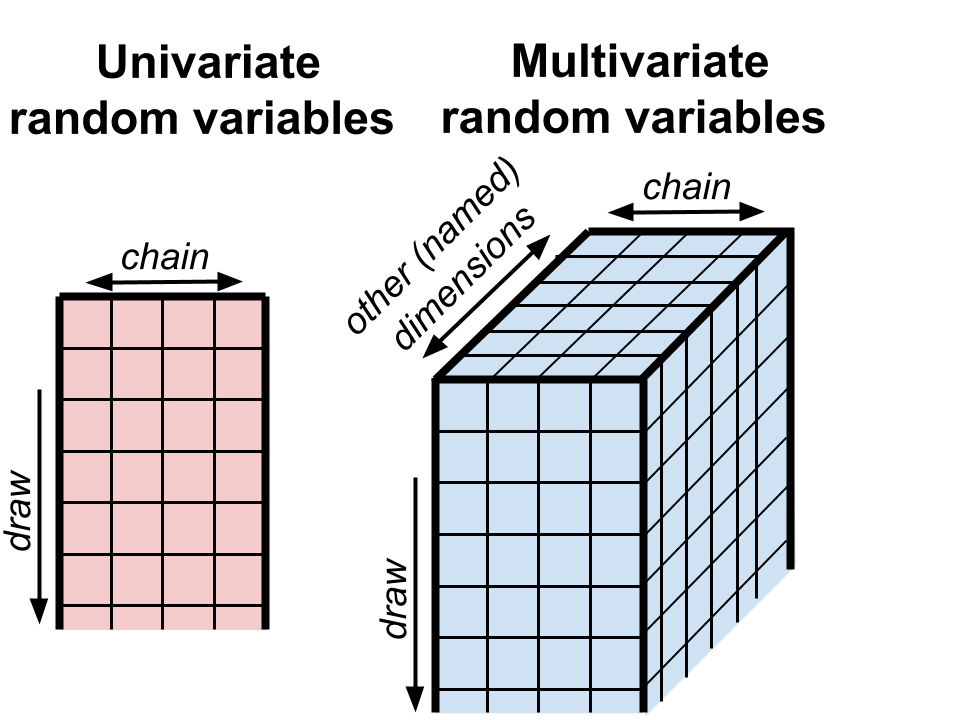
\includegraphics[width=1.0\linewidth]{figures/xarray}
\captionof{figure}{The shape of the xarray objects holding posterior samples for univariate and multivariate random variables}
\end{center}\vspace{1cm}

ArviZ stores these multiple datasets from inference using \textbf{netCDF} groups, which are themselves built with HDF5. The \textbf{InferenceData} class implements this functionality. By using netCDF, in addition to native handling of high dimensional data and being able to use existing serialization and deserialization function, all functions need be implemented only once.

For example, here is how to load data from running 4 chains of NUTS on the radon model of Gelman and Hill using PyMC3.

\begin{lstlisting}
radon = az.load_data('datasets/radon.nc')
Inference data with groups:
	> posterior
	> sample_stats
	> posterior_predictive
	> prior
	> observed_data
\end{lstlisting}

The following plot illustrates ArviZ's ability to work with posterior inferences from many different probabilistic programming libraries.

%----------------------------------------------------------------------------------------
%	plots+diagnostics
%----------------------------------------------------------------------------------------
\section{Plots and Diagnostics}

In addition to common plots for Bayesian analysis like trace plots and forest plots, the library implements many of the visualizations from~\cite{gabry2017visualization}, including ppc plots, pair plots, and parallel coordinate plots. Additionally, it supports a number of statistical checks, such as calculating the effective sample size, the Gelman-Rubin statistic, Pareto-smoothed importance sampling leave-one-out cross validation (PSIS-LOO-CV), and widely applicable information criterion (WAIC).

\begin{center}\vspace{1cm}
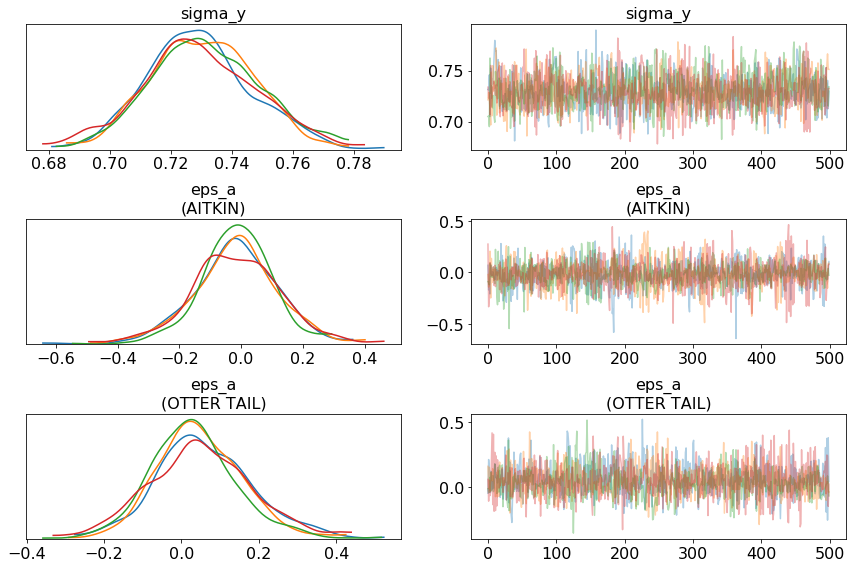
\includegraphics[width=1.0\linewidth]{figures/plot_trace}
\captionof{figure}{\color{Green} A traceplot in ArviZ from the radon example, where the user specified the variable \texttt{eps\_a} and the counties \texttt{AITKIN} and \texttt{OTTER TAIL}.}
\end{center}

\begin{center}\vspace{1cm}
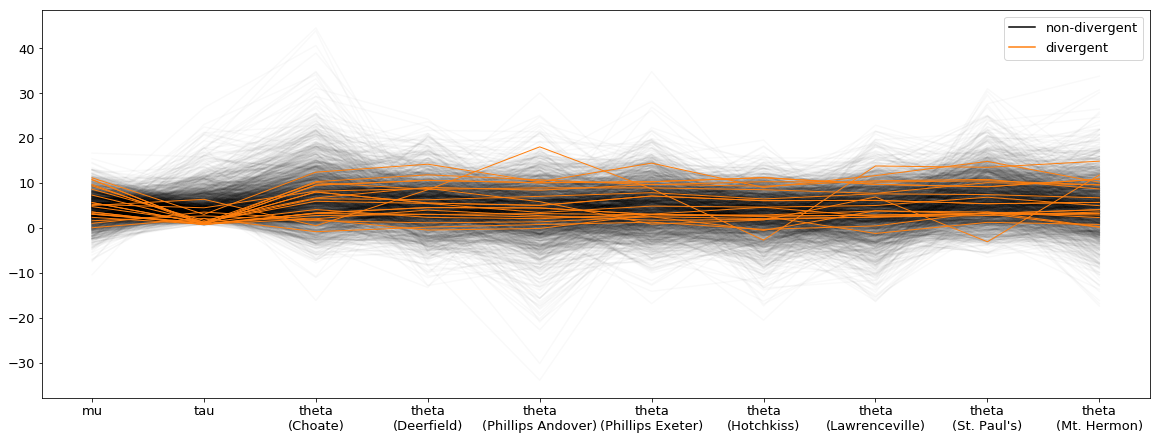
\includegraphics[width=1.0\linewidth]{figures/plot_parallel}
\captionof{figure}{\color{Green} A parallel coordinate plot in ArviZ from the eight schools example, highlighting divergences when tau is small.}
\end{center}

\begin{center}\vspace{1cm}
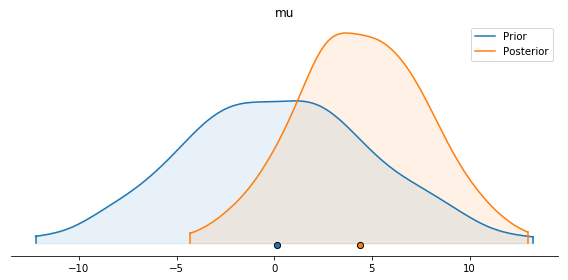
\includegraphics[width=1.0\linewidth]{figures/prior_posterior}
\captionof{figure}{\color{Green}Compoaring the prior and the posterior of a parameter in ArviZ from the eight schools example.}
\end{center}

\begin{center}\vspace{1cm}
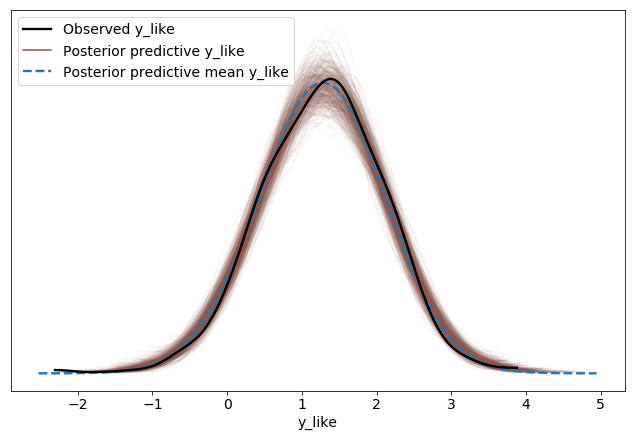
\includegraphics[width=1.0\linewidth]{figures/ppc_plot}
\captionof{figure}{\color{Green} A posterior predictive plot in ArviZ from a Minnesota radon model.}
\end{center}

\begin{center}\vspace{1cm}
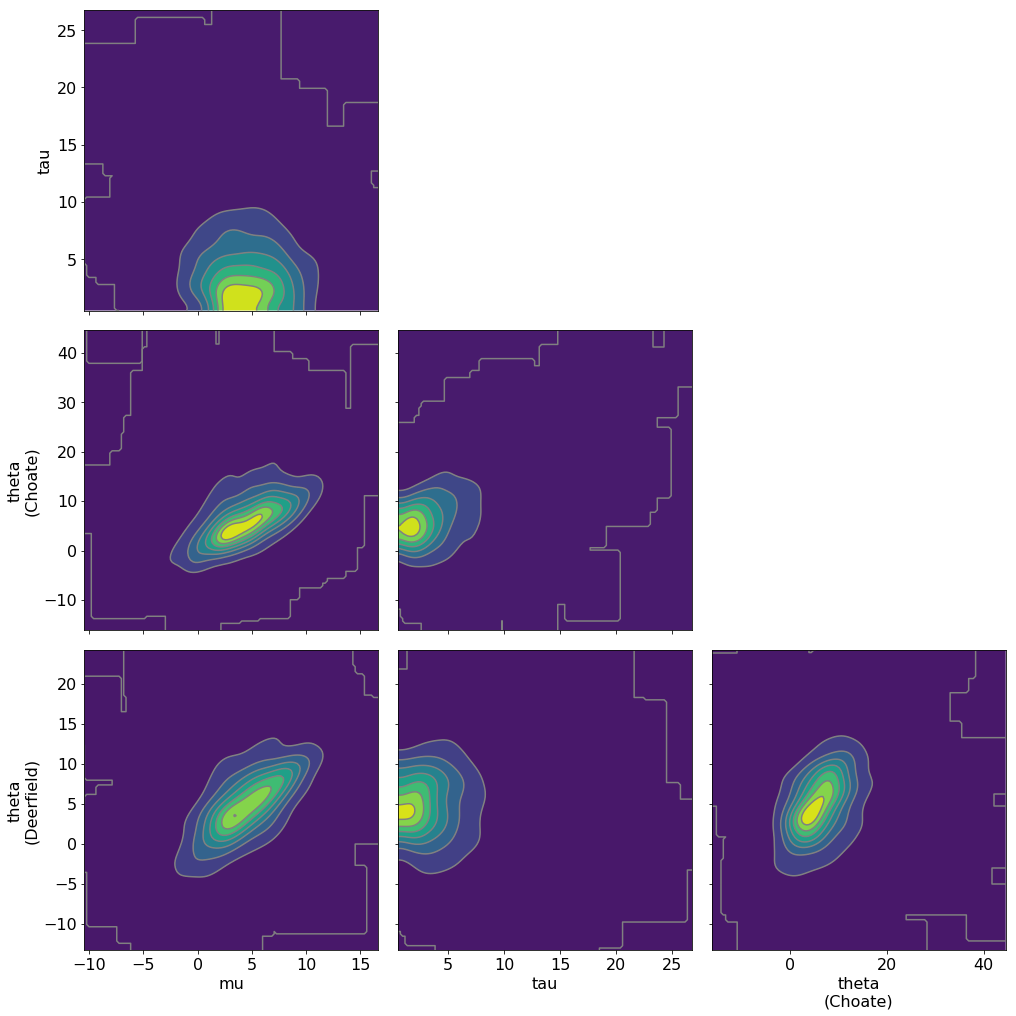
\includegraphics[width=1.0\linewidth]{figures/plot_pair_kde}
\captionof{figure}{\color{Green}A pair plot plot in ArviZ from the eight schools example.}
\end{center}

\begin{center}
\begin{tabular}{lrrr}
\toprule
school           &      mu &   theta &    tau \\
\midrule
Choate           &  199.94 &  452.30 &  213.8 \\
Deerfield        &  199.94 &  514.82 &  213.8 \\
Phillips Andover &  199.94 &  500.70 &  213.8 \\
Phillips Exeter  &  199.94 &  481.20 &  213.8 \\
Hotchkiss        &  199.94 &  397.28 &  213.8 \\
Lawrenceville    &  199.94 &  456.43 &  213.8 \\
St. Paul's       &  199.94 &  537.28 &  213.8 \\
Mt. Hermon       &  199.94 &  561.03 &  213.8 \\
\bottomrule
\end{tabular}
\captionof{table}{\color{Green}Calculating effective samples for a centered eight schools model using ArviZ. Note that the natural output is in an xarray dataset, which may be flattened into the table above.}
\end{center}

%----------------------------------------------------------------------------------------
%	interfaces
%----------------------------------------------------------------------------------------
\section{Interfaces}

\begin{center}\begin{tabular}{|l|l|l|l|}
	\hline
	\textbf{Package} & \textbf{Interface} & \textbf{Sampler stats} & \textbf{Posterior predictive} \\
    \hline
    PyMC3 & Native & Yes & Yes \\
    \hline
    PyStan, CmdStan & Native & Yes & Yes \\
    \hline
    Pyro & Native & No & No \\
    \hline
    Emcee & Native & No & No \\
    \hline
    Edward & Dict & No & No \\
    \hline
\end{tabular}\end{center}\vspace{1cm}

As an explicit example, one may use PyMC3 to sample from the prior predictive, posterior, and posterior predictive distributions, and then convert that into an InferenceData object:

\begin{lstlisting}
with model:
  prior = pm.sample_prior_predictive()
  trace = pm.sample()
  ppc = pm.sample_posterior_predictive(trace)

radon = arviz.from_pymc3(
  trace=trace,
  prior=prior,
  posterior_predictive=ppc,
  coords={
    'county': mn_counties,
    'observed_county': observed_counties
  },
  dims={
      'eps_a': ['county'],
      'a': ['observed_county'],
      'mu_a': ['observed_county'],
      'y_like': ['observed_county']
  })
\end{lstlisting}

This creates the radon data from the first section. While we specified certain parts of the data, note that ArviZ also used the available objects to extract observed data, which is an attribute on the trace, and sample stats, which records metrics like energy, tree depth, and whether there was a divergence. These are indexed using the same ``draw'' and ``chain'' dimensions that the other parameters use, simplifying queries.

\begin{center}\vspace{1cm}
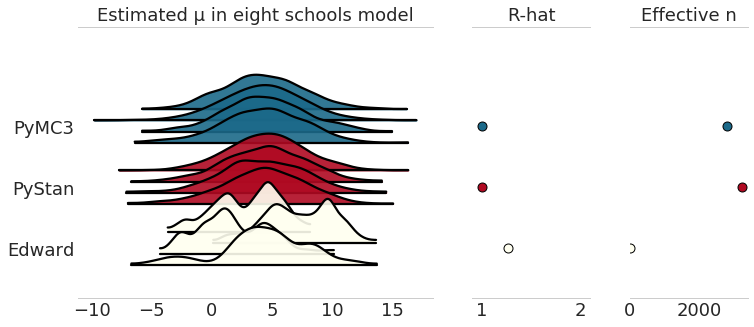
\includegraphics[width=1.0\linewidth]{figures/forestplot}
\captionof{figure}{\color{Green} An example ridgeplot in ArviZ comparing estimates from the same model in three libraries, suggesting a poorly tuned sampler from Edward}
\end{center}


 %----------------------------------------------------------------------------------------
%	REFERENCES
%----------------------------------------------------------------------------------------

\section{Acknowledgements}

The ArviZ project is open source, but has seen significant contributions from Osvaldo Martin, Ari Hartikainen, Ravin Kumar, and Adrian Seyboldt.

\section{References}
\begin{center}{\color{Green}http://arviz-devs.github.io/arviz}\end{center}

The following QR code links to a Jupyter notebook containing the ArviZ code necessary to reproduce the plots in this poster.


\begin{center}\vspace{1cm}

\includegraphics[width=0.5\linewidth]{figures/qr}
\end{center}

% \nocite{*} % Print all references regardless of whether they were cited in the poster or not
\vspace{-3cm}
\renewcommand{\refname}{}
\bibliographystyle{plain} % Plain referencing style
\bibliography{/home/colin/projects/probprog/poster/arviz} % Use the example bibliography file sample.bib
%----------------------------------------------------------------------------------------

\end{multicols}
\end{document}